\chapter{Formation des 'petites' structures}
\newthought{Une surdensité de matière} va nécessairement sortir du régime des faibles valeurs au bout d'un certain temps : le mécanisme d'instabilité gravitationnelle va condenser les structures vers des grandes densités et le jeu d'équations linéarisées utilisé dans le chapitre précédent n'est plus valable. Nous allons ici développer un modèle simple de surdensité qui permet de suivre l'évolution d'une telle structure en effondrement \index{effondrement sphérique}. Le destin d'une telle structure est de finir en halo de matière\index{halo}\sidenote{et donc dominé par la matière noire} à l'équilibre, dont on exposera aussi les propriétés de base. A des fins de simplification, nous allons par la suite nous limiter au cas d'un Univers rempli uniquement de matière noire, non-collisionnelle, avec $\Omega_m=1$. Comme vu précédemment, cet Univers de Einstein-de Sitter\index{Einstein- de Sitter} est régi par une expansion en :
\begin{equation}
a(t) \sim t^{2/3}.
\end{equation}

\section{Au-delà du régime linéaire : le modèle d'effondrement sphérique\index{effondrement sphérique}}

Considérons une surdensité, sphérique de rayon $r$, baignant dans un Univers de densité $\bar \rho$. A l'intérieur de cette surdensité, la densité est initialement légèrement plus grande que celle du fond avec $\rho = (1+\delta) \bar \rho$ et uniforme à l'intérieur de ce rayon \sidenote{On parle aussi de modèle 'chapeau haut-de-forme' \index{haut-de-forme} à cause du profil de densité en créneau associé }.  Ce modèle ressemble grandement au modèle de cosmologie newtonienne \index{cosmologie newtonienne} abordé en début d'ouvrage : dans ce modèle de cosmologie et pour la surdensité qui nous intéresse, sa dynamique est régie uniquement par la matière qui se trouve à l'intérieur et la couche la plus externe de la surdensité suit le principe fondamental de la dynamique\index{principe fondamental de la dynamique} :
\begin{equation}
\ddot r = -\frac{GM(<r)}{r^2}.
\end{equation}
Rappelons que $r(t)=a(t)r_0$ et dans le cas où cette couche est en expansion infinie \sidenote{ avec $\dot a >0$}, on peut facilement intégrer l'équation différentielle précédente pour obtenir :
\begin{eqnarray}
\dot a &=&\sqrt{\frac{2GM(<r)}{ar_0^3}}\\
r(t)&=&\left(\frac{9GM(<r)}{2}\right)^{1/3} t^{2/3}
\end{eqnarray}
avec une dépendance temporelle en $t^{2/3}$ conforme au modèle Einstein - de Sitter\index{Einstein-de Sitter}. Toutefois, cette dépendance ne peut représenter l'effondrement d'une structure, puisqu'on attend d'elle que son rayon diminue au delà d'un certain temps\sidenote{donc l'hypothèse $\dot a >0$ ne tient plus et nous empêche d'intégrer simplement l'équation différentielle}.

\newthought{Un bon point de départ} est l'équation de conservation de l'énergie spécifique de la couche externe de notre structure :
\begin{equation}
E=\frac{\dot r^2}{2}-\frac{GM}{r}
\end{equation}
où $M=M(<r)$ désigne la masse à l'intérieur de la couche la plus externe. Rappelons que dans ce type de modèle les couches ne se croisent pas \sidenote{comme indiqué par $r(t)=a(t)r_0$ : une couche externe reste toujours une couche externe} et cette masse interne $M$ reste constante. Enfin, notre structure est vouée à s'effondrer, son énergie mécanique\index{energie!mécanique} totale est donc négative, $E<0$. Dans ce type de situation, on peut montrer que la solution $r(t)$ s'exprime sous forme \textit{paramétrique} (voir aussi la figure \ref{f:rtparam}):
\begin{eqnarray}
r(\theta)&=&A (1-\cos \theta)\\
t(\theta)&=&B (\theta-\sin \theta)
\end{eqnarray}
où $\theta$ est un paramètre tel que $\theta \in [0,2\pi]$. La vitesse de la couche peut également s'écrire sous forme paramétrique\sidenote{obtenue en dérivant l'équation sur le temps puis en l'injectant dans celle sur le rayon}:
\begin{equation}
v(\theta)=\dot r= \frac{A \sin \theta}{B(1-\cos \theta)}.
\end{equation}
Ici, $A$ et $B$ sont respectivement des rayons et temps caractéristiques du problème traité avec :
\begin{eqnarray}
A&=&\frac{GM}{2|E|}\\
B&=&\frac{GM}{(2|E|)^{3/2}}\\
A^3&=&GM B^2
\end{eqnarray}
où la dernière relation est similaire à la troisième loi de Kepler qui relie période et rayon des orbites autour d'un corps massif.


\begin{figure}[htbp]
	\centering
		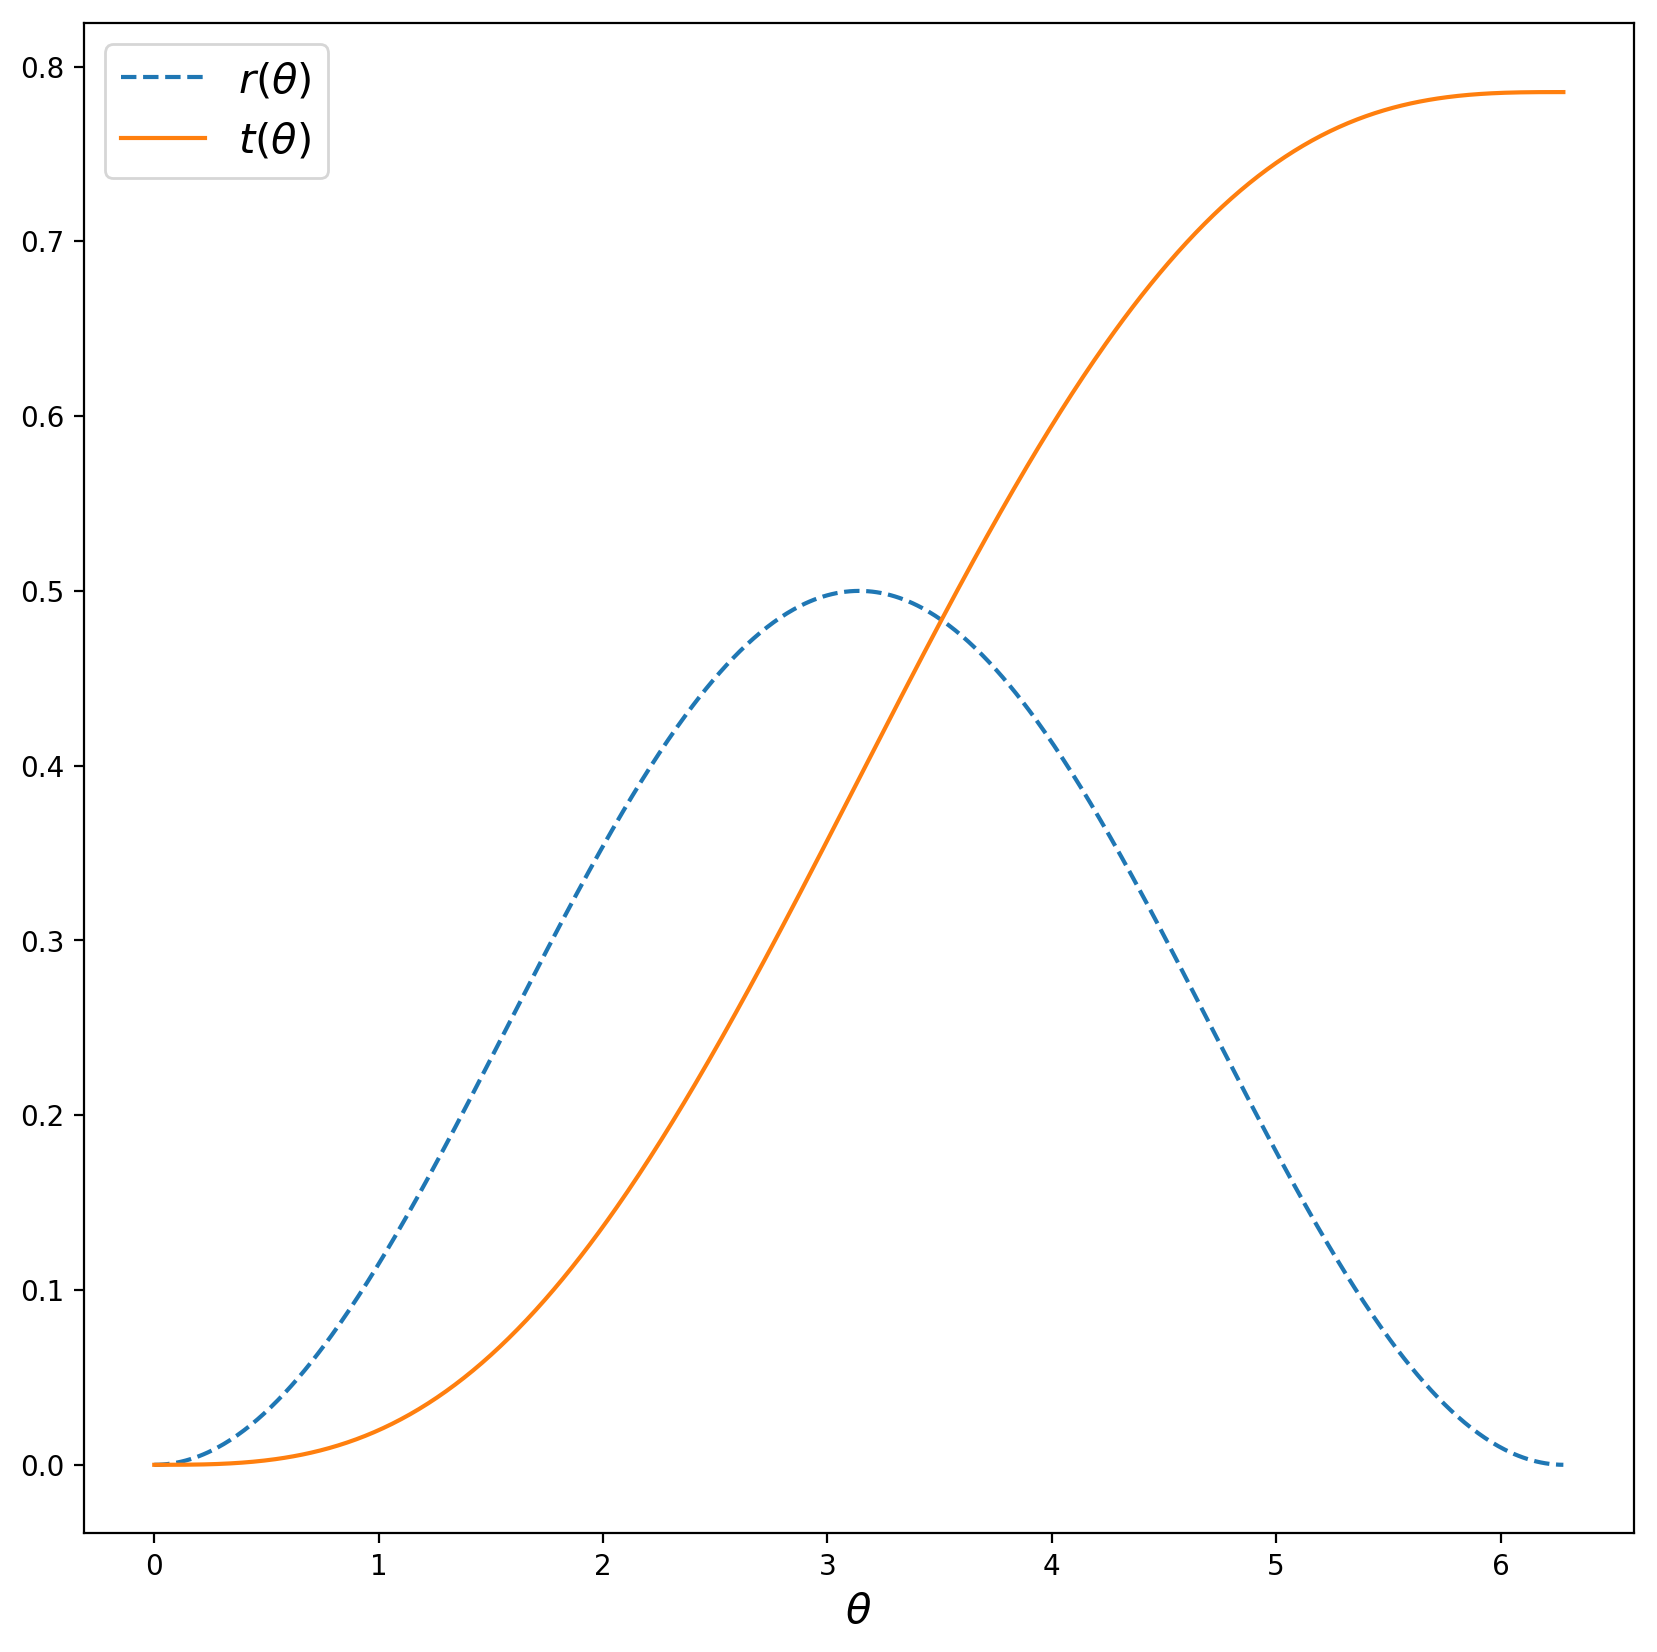
\includegraphics[height=10cm]{figs/rtparam.png}
		\caption[Les solutions paramétriques de l'effondrement sphérique]{Les solutions du modèle d'effondrement sphérique en fonction du paramètre $\theta$. Le temps $t$ est une fonction monotone de ce paramètre tandis que le rayon de la surdensité passe par un maximum, correspondant au découplage de la structure par rapport au fond cosmologique, avant de tendre vers 0 à la fin de l'effondrement.}
	\label{f:rtparam}
\end{figure}

Ces relations paramétriques permettent de caractériser les grandes étapes du processus d'effondrement. D'abord, on constate que l'évolution du rayon n'est pas monotone, celui-ci croît, atteint un maximum et décroit pour devenir nul : notre surdensité évolue d'abord avec le fond, suivant l'expansion globale, puis elle atteint une extension maximale avant de se \textit{découpler} du flot global. La structure se réduit en taille avant d'atteindre une extension nulle et par conséquent sa densité devient infinie ! Cette évolution \sidenote{qui est la même que celle d'un Univers de densité supérieure à la densité critique} conduit naturellement à des régimes de densité non linéaires\index{régime non-linéaire}. Par simple inspection, on constate que le découplage\index{expansion!découplage}, correspondant au maximum de $r$, opère pour $\theta=\pi$ et 
\begin{eqnarray}
r_d&=&2A\\
t_d&=&\pi B.
\end{eqnarray}
L'effondrement final correspond quant à lui à $\theta=2 \pi$ et 
\begin{eqnarray}
r_e&=&0\\
t_e&=&2\pi B.
\end{eqnarray}
Le temps nécessaire à l'effondrement\index{effondrement sphérique} \sidenote{on utilise aussi fréquemment les termes anglais de \textit{turn-around} pour le découplage et de \textit{collapse} pour l'effondrement} total de la structure est le double de celui nécessaire au découplage : $t_e=2 t_d$.

\newthought{La surdensité varie aussi de façon paramétrique}. La densité à l'intérieur de la structure est donnée par :
\begin{equation}
\rho = \frac{M}{4/3 \pi r^3}=\frac{3M}{4\pi A^3(1-\cos \theta)^3}, 
\end{equation}
tandis que la densité du fond, égale à la densité critique dans notre modèle est donnée par \sidenote{on rappelle que $H=\frac{\dot a}{a}$ et $a\sim t^{2/3}$ dans Einstein- de Sitter}:
\begin{equation}
\bar \rho =\frac{3H^2}{8\pi G}=\frac{1}{6\pi G t^2}=\frac{1}{B^2 6\pi G (\theta-\sin \theta)^2}.
\end{equation}
On obtient alors la formulation paramétrique de l'évolution de la surdensité :
\begin{equation}
\frac{\rho}{\bar \rho}=1+\delta=\frac{9}{2}\frac{(\theta - \sin \theta)^2}{(1-\cos \theta)^3}.
\label{e:dcoll}
\end{equation}
Bien sûr, cette équation ne rend pas compte des phases ultimes de l'effondrement : cet effondrement doit s'arrêter lorsqu'un équilibre est atteint après réorganisation de la matière et des vitesses. Les coquilles se croisent\index{croisement de coquille}, la masse à l'intérieur de la coquille change et de l'énergie est échangée entre les couches.  

Toutefois, une bonne approximation du processus à l'œuvre peut être obtenue en invoquant le théorème du viriel\index{théorème du viriel}. Une fois l'équilibre atteint, notre couche externe doit satisfaire
\begin{equation}
2 T +U = 0,
\end{equation}
où $T$ et $U$ désignent respectivement l'énergie cinétique\index{energie cinétique}\index{energie potentielle} et potentielle de notre couche externe après viriélisation. Comme par ailleurs l'énergie reste conservée, l'énergie totale en fin de viriélisation est donnée par:
\begin{equation}
E=\frac{U}{2}=-\frac{GM}{2r_v}
\end{equation}
où l'on considère que la masse interne n'a pas été modifiée significativement par la redistribution. A l'équilibre, la couche ne bouge plus et son énergie totale est complètement définie par son énergie potentielle. C'est également le cas lors du découplage, durant lequel l'énergie cinétique est nulle par définition et \sidenote{en effet le découplage correspond au maximum d'extension de la surdensité avec $\dot r=0$ par définition}
\begin{equation}
E=-\frac{GM}{r_d}.
\end{equation}
Par conservation de l'énergie de la couche et en combinant ces deux derniers résultats, on obtient une relation entre le rayon de la couche externe à l'équilibre $r_v$ et celui lors du découplage $r_d$:
\begin{equation}
r_v\sim \frac{1}{2}r_d,
\end{equation}
le rayon de la structure se stabilise autour d'une valeur correspondant à la moitié du rayon lors du découplage. Ce rayon final est aussi appelé \textit{rayon de viriel}\index{rayon de viriel}, et est utilisé de façon générique pour désigner les bords 'externes' d'un halo de galaxie.

On peut également évaluer la valeur de la surdensité finale après la phase de viriélisation. On cherche à évaluer
\begin{equation}
1+\delta_\mathrm{v}=\frac{\rho(t_v)}{\bar \rho(t_v)},
\end{equation}
ce qui nécessite d'évaluer les deux densités $\rho$ et $\bar \rho$ post-viriélisation. La densité du fond est simple à obtenir, car la viriélisation opère au temps $t_v=t_e=2t_d=2\pi B$, on obtient donc:
\begin{equation}
\bar \rho(t_v) = \frac{1}{6\pi G t_v^2}=\frac{1}{4}\bar \rho (t_d).
\end{equation} 
De même, sachant que le rayon de viriel est la moitié du rayon de découplage, il existe une relation simple\sidenote{sachant que $r_v=r_d/2$} entre la densité à l'équilibre et celle lors du découplage:
\begin{equation}
\rho(t_v)=\frac{3 M}{4\pi r_v^3}=8 \rho(t_d)
\end{equation}
d'où la relation :
\begin{equation}
1+ \delta_v=\frac{8 \rho(t_d)}{\frac{1}{4}\bar \rho (t_d)}=32(1+\delta_d).
\end{equation}
Sachant que le découplage opère pour $\theta =\pi$, l'évaluation de l'équation \ref{e:dcoll} pour cette valeur donne $\delta_d\sim 5.55$ et une valeur de densité à l'équilibre 
\begin{equation}
1+\delta_v \sim 178.
\end{equation} 
En résumé, une structure qui s'effondre sous l'effet de l'instabilité gravitationnelle voit sa densité se stabiliser autour de 200 fois celle du fond. Pour cette raison, on désigne fréquemment le rayon de viriel $r_v$\index{rayon de viriel} sous le terme de $r_{200}$ et par exemple, c'est comme cela qu'on détermine l'extension d'un halo de galaxie dans une simulation numérique : son extension est choisie de telle façon à ce que la surdensité interne soit proche de 200.

\newthought{On peut également proposer une extrapolation linéaire\index{effondrement sphérique!extrapolation linéaire}} du calcul qui vient d'être réalisé. Il s'agit de calculer la surdensité au moment de l'effondrement mais telle qu'elle est prédite dans le régime linéaire. L'intérêt d'un tel calcul est qu'il permet de prédire simplement les régions qui vont s'effondrer sans avoir à réaliser un calcul non-linéaire complet : en se donnant un champ de densité, on peut prédire aisément sa croissance linéaire et désigner quelles régions vont s'effondrer et à quel instant. Si l'on reprend notre modèle paramétrique, le régime des faibles perturbations est celui qui opère au début, donc quand $\theta \ll 1$. Ce paramètre devient alors une simple fonction de $t$\sidenote[][-2cm]{obtenu via un développement limité de $t(\theta)$} :
\begin{equation}
\theta \sim \left(\frac{6t}{B}\right)^{1/3}.
\end{equation}
De même dans ce régime et en utilisant les bons développements limités
\sidenote{on rappelle que $\cos \theta \sim 1-\theta^2/2+\theta^4/24$ et $\sin \theta \sim \theta -\theta^3/6 +\theta^5/120$.}
, l'équation \ref{e:dcoll} peut être réécrite :
\begin{equation}
1+\delta =\frac{9}{2}\frac{(\theta -\sin \theta)^2}{(1-\cos \theta)^3}\sim 1+\frac{3}{20} \theta^2.
\end{equation}
D'où l'expression de $\delta_l$ dans le régime linéaire en fonction du temps:
\begin{equation}
\delta_l=\frac{3}{20}\left(\frac{6t}{B}\right)^{2/3}=\frac{3}{20}(6\pi)^{2/3}\left(\frac{t}{t_d}\right)^{2/3}.
\end{equation}
On note d'ores et déjà que l'on retrouve la fameuse dépendance en $t^{2/3}$, propre aux modèles dominés par la matière. Au moment de l'effondrement, $t=t_e=t_v=2t_d$, ce qui donne $\delta_l=1.69$. Cette valeur revêt un caractère un peu 'magique' pour les cosmologues : si on évolue un champ de densité linéairement, les régions qui dépassent ce seuil vont s'effondrer. Ce type de raisonnement permet de prédire quelles régions vont former des structures et à quel instant : c'est ce qui permet par exemple de faire des prédictions analytiques sur la fonction de masse des halos de matière noire\sidenote{voir le chapitre dédié à la matière noire} ou bien sur leur histoire de formation. Ce types de prédictions sont à la base de modèles \textit{analytiques} de formation des galaxies où la connaissance de l'histoire de formation de ces objets obtenue par cette méthode peut être utilisée pour prédire l'évolution des baryons en leur sein et les propriétés des galaxies qui s'y forment.

\begin{figure}[htbp]
	\centering
		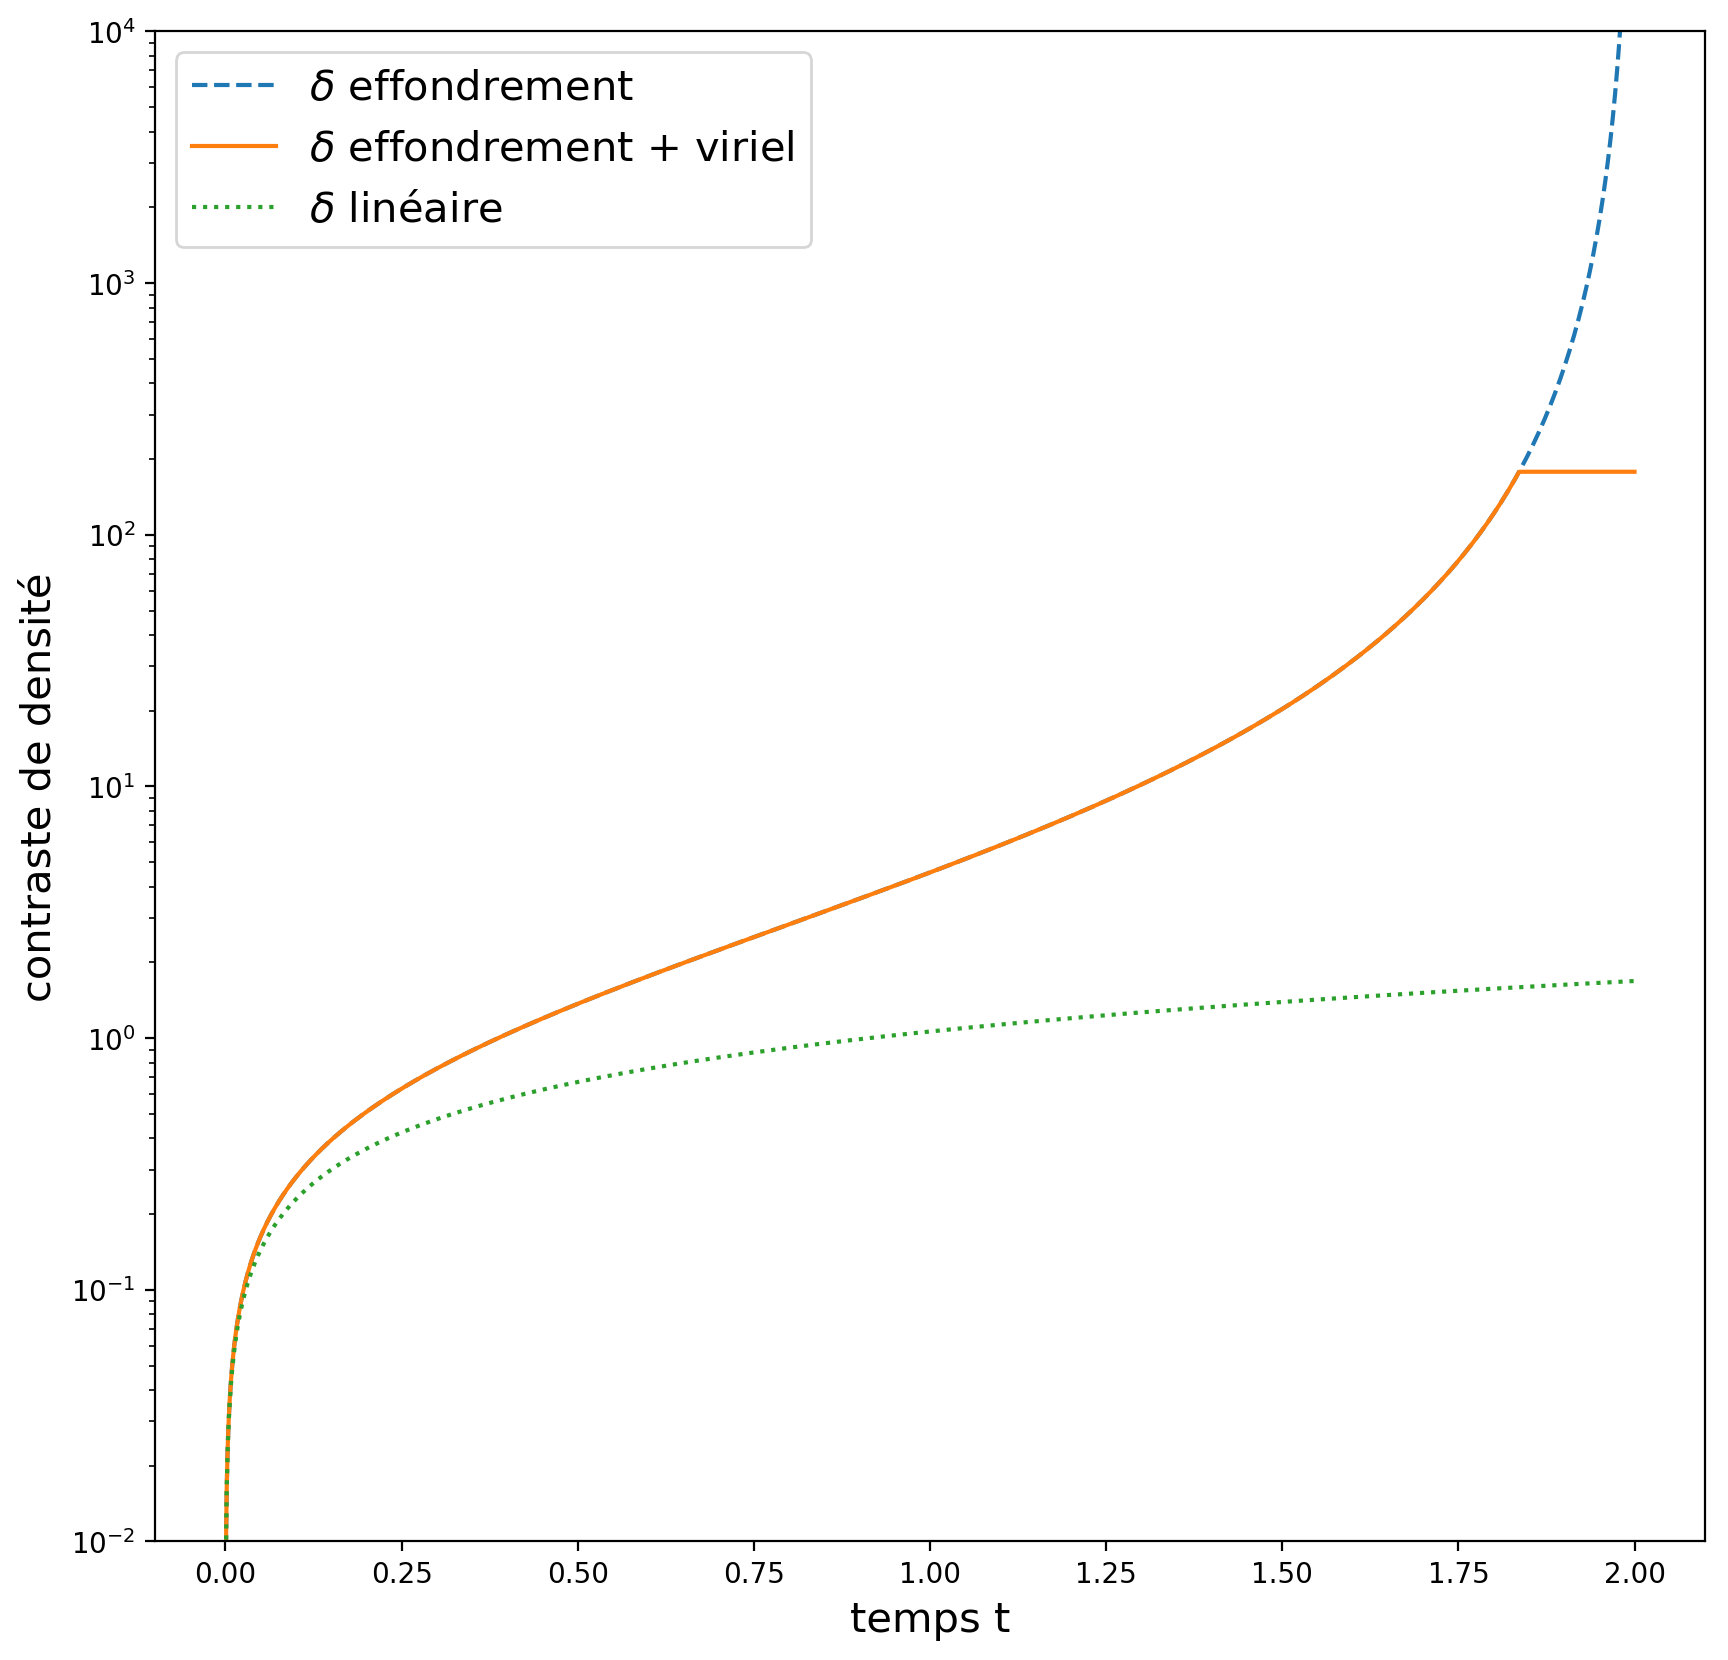
\includegraphics[height=10cm]{figs/delta_coll.png}
		\caption[Évolution temporelle du contraste de densité pour l'effondrement sphérique]{
		Les différentes solutions pour le contraste de densité $\delta=\rho/\bar \rho -1$ au cours du temps. On constate que le contraste non-linéaire évolue vers une singularité au moment de l'effondrement, la densité tend vers l'infini. Pratiquement, la surdensité va se stabiliser autour d'un contraste d'environ 200, correspondant à un état d'équilibre issu d'une redistribution de la matière et des vitesses appelée viriélisation. L'approximation linéaire
		 suit la solution non-linéaire dans le régime des petits contrastes mais évolue plus lentement aux temps ultérieurs pour atteindre une valeur de 1.68 au moment où la structure devrait s'effondrer.
		}
	\label{f:dcoll}
\end{figure}


\section{Propriétés générique des halos post-effondrement}
Les structures effondrées étudiées ici sont de fait les halos de matière noire\index{halo} qui entourent les galaxies. Nous venons par exemple de prédire que la densité typique interne à ces objets doit être de l'ordre de 200 fois celle du fond, mais qu'en est-il du profil de densité de ces halos ? Les simulations cosmologiques montrent que le profil résultant de la viriélisation est de forme \textit{ universelle} et qu'une forme fonctionnelle simple permet d'ajuster le profil de la distribution de matière sur des grandes gammes de masses d'objet. La plus célèbre de ces formes fonctionnelles est le profil NFW\index{profil NFW} \sidenote{du nom de ses découvreurs Navarro, Frenk et White} : 
\begin{equation}
\rho(r)=\frac{\rho_s}{(r/r_s)(1+r/r_s)^2}.
\end{equation}

\begin{figure}[htbp]
	\centering
		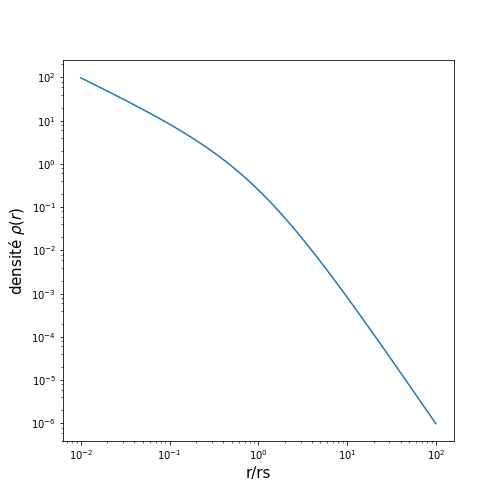
\includegraphics[height=9cm]{figs/nfw.png}
		\caption[Le profil de densité NFW]{Le profil de densité de NFW est le profil universel des halos de matière noire mesuré dans les simulations de formation des grandes structures. Ce profil se caractérise par le 'pic' en $r^{-1}$ au centre : ce type de distribution de matière n'est pas observé dans la cinématique des étoiles centrales des galaxies naines par exemple, posant difficulté aux prédictions des modèles de matière noire. L'injection répétée d'énergie dans le gaz central pourrait conduire à une redistribution de la matière dans ces régions, y compris dans la composante matière noire, pour 'aplatir' ce profil.}
	\label{f:nfw}
\end{figure}

Ce profil se comporte en $r^{-3}$ à grande distance et en $r^{-1}$ près du centre du halo et on qualifie ce profil de 'piqué'\sidenote{d'autres profils avec davantage de degrés de liberté qui ajustent mieux le comportement central (profil d'Einasto par exemple) montrent que ce comportement piqué tend tout de même à s'affaisser dans les régions les plus internes }. Le rayon $r_s$ est le rayon de transition entre ces deux régimes de pentes à courte et grande distance. Les mêmes simulations montrent que le rapport entre ce rayon de transition et le rayon de viriel étudié précédemment, appelé aussi concentration\index{halo!concentration}, est de l'ordre de :
\begin{equation}
c=\frac{r_v}{r_s}\sim 10
\end{equation}
sachant que les petits halos sont plutôt plus concentrés que cette valeur et les plus massifs sont plutôt moins concentrés. Ce comportement piqué au centre n'est pas sans poser problèmes car les observations de la cinématique du centre des galaxies naines semblent indiquer un profil de densité possédant plutôt un cœur plat \sidenote{avec des profils en $\rho \sim r^0$ }. Bien que cela soit encore un sujet de recherche actif, le consensus grandissant est que la physique baryonique, et notamment les processus d'injection d'énergie répétée dans le gaz par les générations successives de supernovæ\index{supernova} au centre des halos, conduirait à une redistribution des profils centraux de matière vers des profils à 'cœur' : c'est l'absence de prise en compte de ces effets dans les simulations qui conduirait à cette différence entre modèles et observations.


\begin{figure}[htbp]
	\centering
		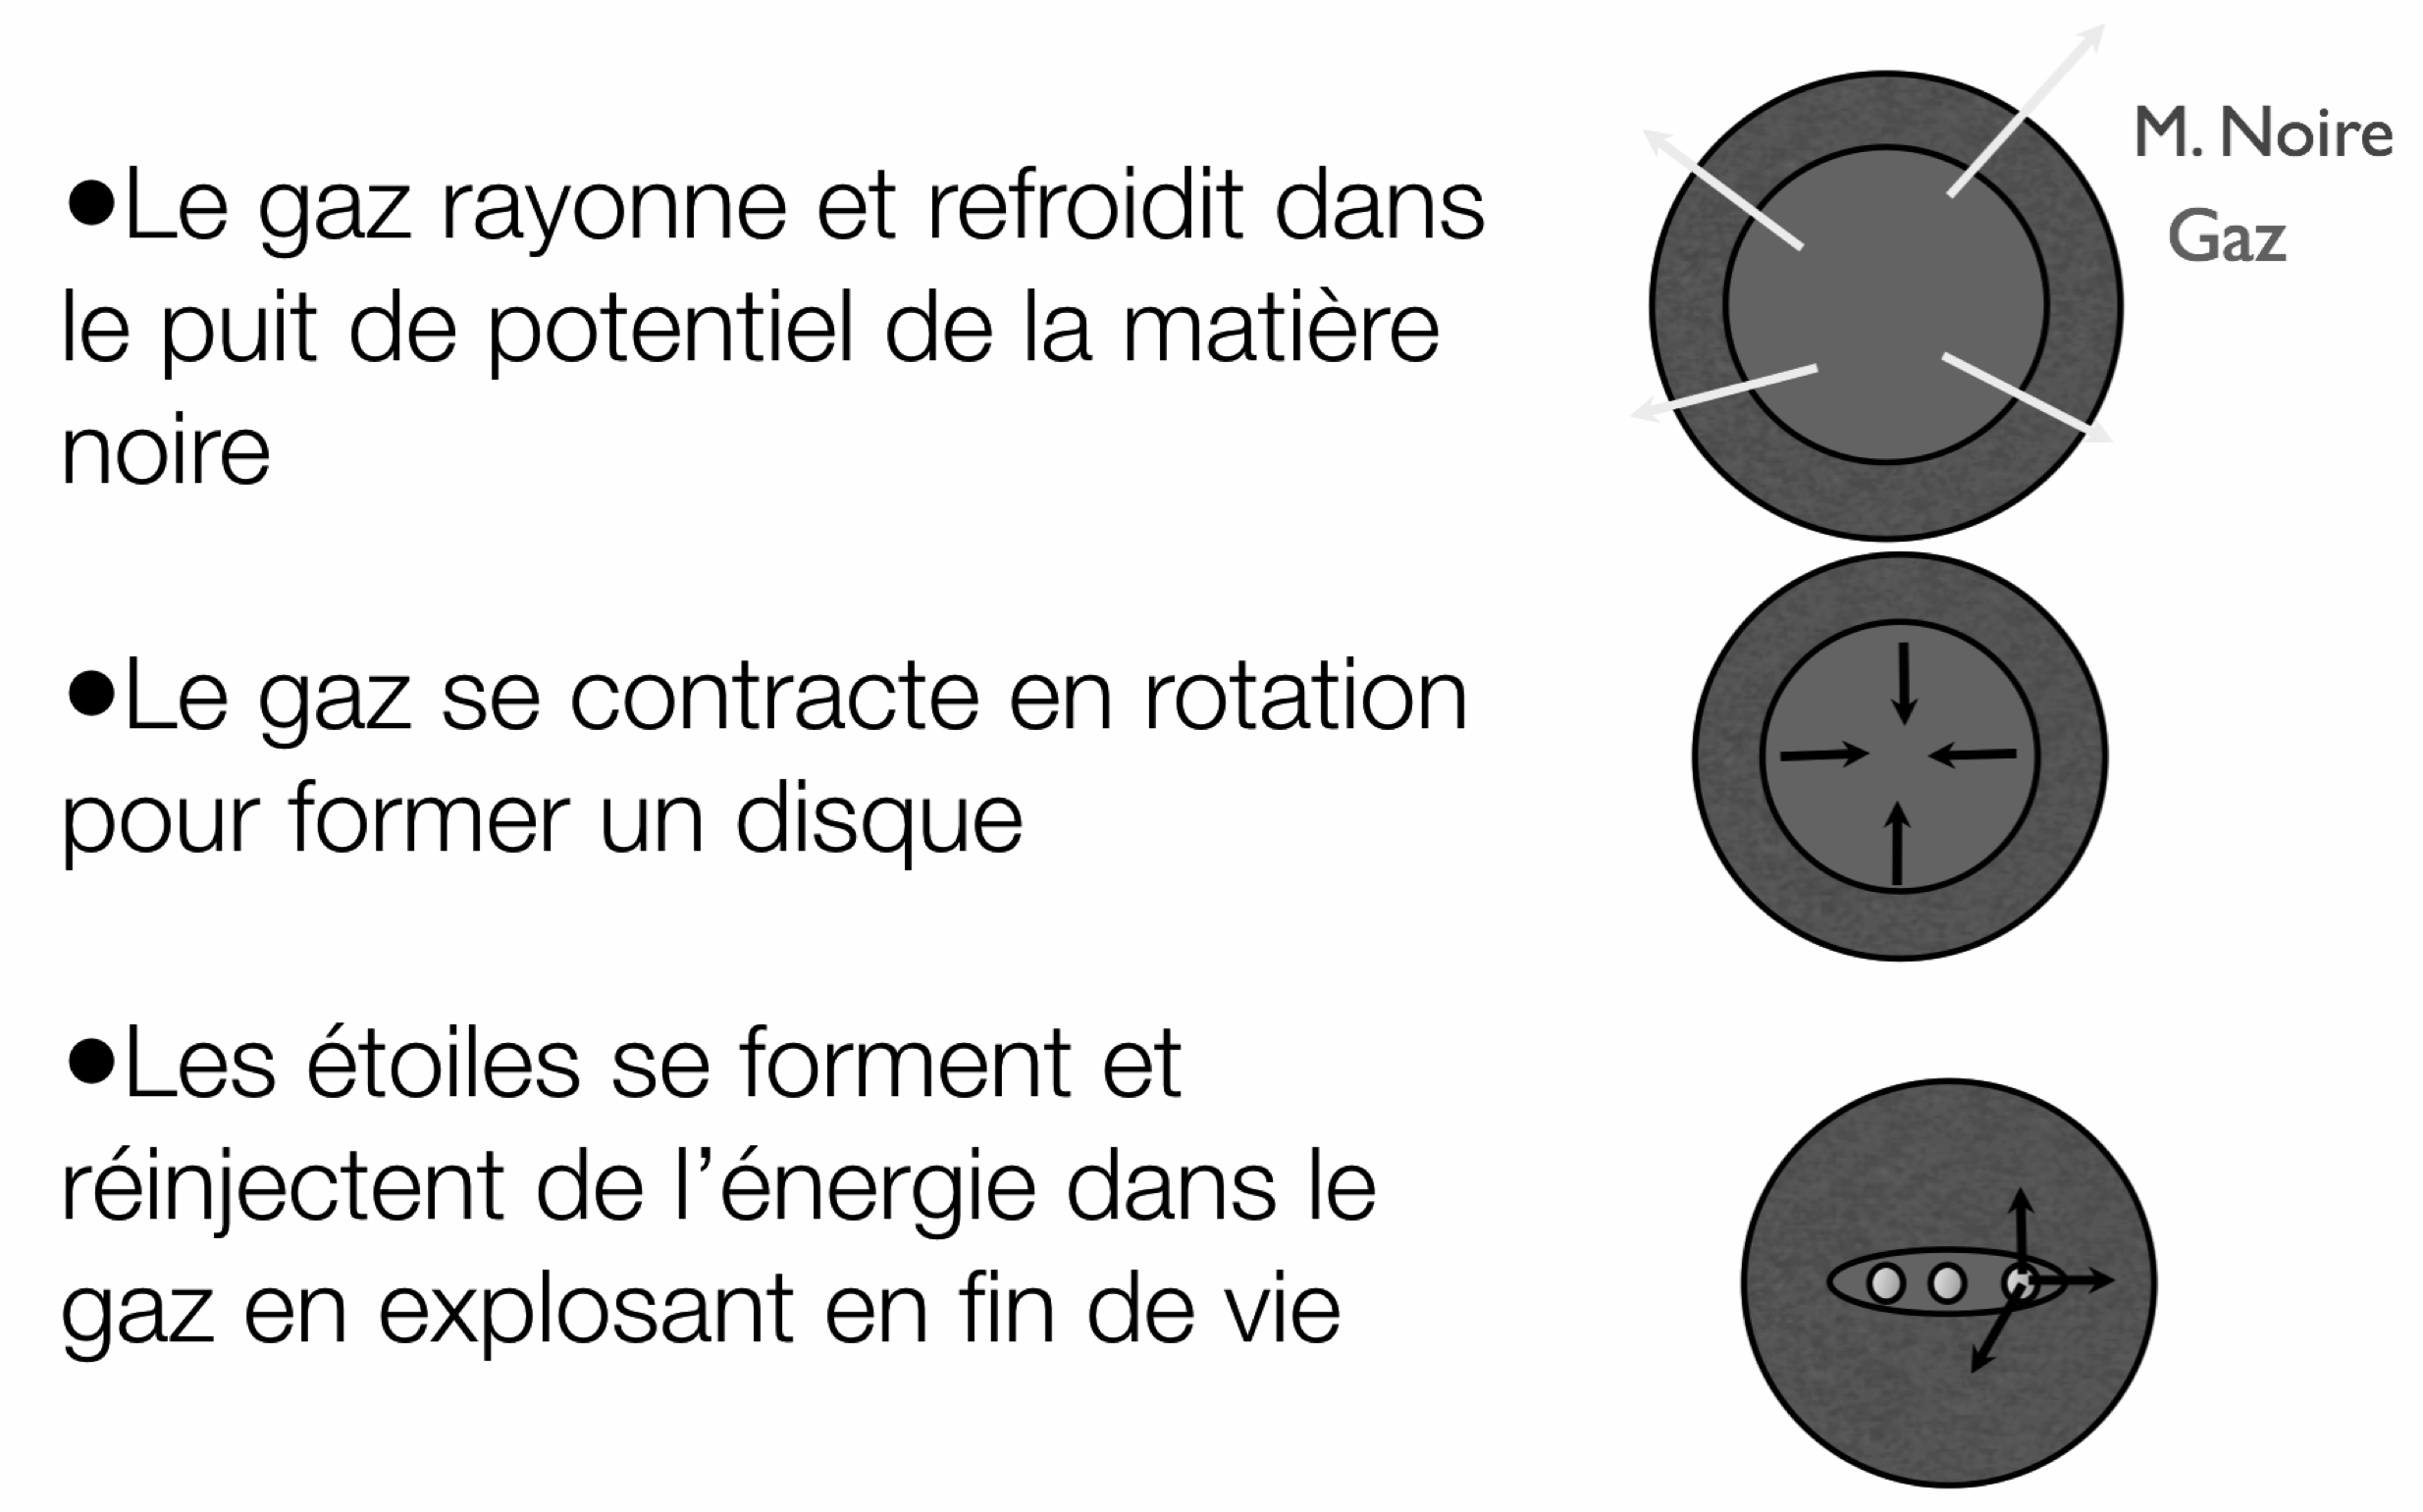
\includegraphics[height=10cm]{figs/coolgal.png}
		\caption[Formation schématique d'une galaxie]{Schéma de la formation d'une galaxie. Dans un premier temps, le gaz évacue de l'énergie interne (refroidissement) dans son halo de matière noire en rayonnant. Ensuite il se contracte pour atteindre des hautes densités : la rotation initiale du gaz est conservée et conduit naturellement à des disques tournants. Enfin, les régimes de densité permettant la formation stellaire se mettent en place dans la galaxie et en fin de vie les étoiles explosent en supernovæ et réchauffe le gaz. }
	\label{f:coolgal}
\end{figure}


\newthought{Le gaz n'est pas en reste} dans le processus de viriélisation. Une fois l'équilibre atteint, le gaz va aussi s'organiser dans le potentiel gravitationnel du halo dominé par la matière noire. On peut par exemple lui assigner une température d'équilibre appelée aussi température de viriel\index{température!de viriel}. Conformément au théorème du viriel\index{théorème du viriel}, l'équipartition entre énergie cinétique et potentielle des baryons peut s'écrire:
\begin{equation}
3\frac{M_gk_B T}{\mu m_p} - \alpha \frac{G M_v M_g}{r_v}=0.
\end{equation}
Ici $\mu mp$ désigne la masse typique d'une particule (atome d'hydrogène, hélium, électron), $M_g$ est la masse de gaz totale et $\alpha$ est un facteur de forme proche de l'unité dépendant du profil de masse du gaz. La température de viriel du gaz est donc une fonction simple de la masse et de la taille du halo : $T_v\sim M_v/r_v \sim V_v^2$ \sidenote{ici $V_v=\sqrt{GM_v/r_v}$ désigne la vitesse du viriel, la vitesse circulaire au rayon de viriel, qui est une mesure de sa masse. }, et pour une masse de halo donnée cela implique que si un processus quelconque (comme l'arrivée de rayonnement) chauffe le gaz au dessus de cette température, celui-ci ne peut rester à l'équilibre et éventuellement s'évaporer. Bien sûr la température du gaz à l'intérieur d'une vraie galaxie n'est pas constante et cette température de viriel n'est qu'une estimation des régimes typiques des températures atteintes au sein des halos.

Toutefois, un gaz dispose d'un canal d'évacuation d'énergie interne inaccessible à la matière noire : les processus baryoniques régis par les interactions électromagnétiques, dont en particulier la production de rayonnement qui peut emporter de l'énergie interne du gaz. On appelle ces processus des \textit{processus de refroidissement}\index{fonction de refroidissement}, caractérisé par une fonction de refroidissement $\Lambda(x,T)$ qui dépend de la température du gaz $T$ et de sa fraction d'ionisation $x$\sidenote{$x=1$ désigne un gaz dont tous les atomes sont ionisés, $x=0$ où ils sont tous neutres}. La quantité d'énergie évacuée par le gaz, en $J/m^3/s$, est donnée par :
\begin{equation}
\Delta e_\mathrm{int}=n_H^2 \Lambda(x,T),
\end{equation}
où $n_H$ désigne la densité d'atomes disponibles.
Cette fonction de refroidissement dicte la quantité d'énergie évacuée à chaque instant par les processus atomiques d'excitation collisionnelle, d'ionisation, de recombinaison et de brehmstrahlung : tous ces processus dépendent du nombre d'atomes neutres et d'électrons disponibles, d'où la dépendance de la fonction de refroidissement en fraction d'ionisation et en $n_H$. Ces processus de refroidissement produisent de la lumière, font diminuer l'énergie interne du gaz qui perd en support thermique et peut donc se contracter davantage : le gaz va devenir de plus en plus dense dans un halo\index{halo} de matière noire qui lui va rester à l'équilibre de viriel. Par ailleurs, la conservation du moment angulaire\index{moment angulaire} du gaz fait que toute rotation initiale de ce dernier, même faible, est maintenue et conduit naturellement à la formation de disques en rotation. 
La conséquence ultime de ce processus de condensation est la formation d'une galaxie et au sein de celle-ci la formation d'étoiles. Bien sûr, si le refroidissement n'est pas assez efficace, le gaz va retrouver son équilibre hydrostatique et l'effondrement du gaz n'aura pas lieu : la compétition entre ces deux effets s'évalue en comparant les temps de refroidissement\index{temps! de refroidissement} et de rééquilibrage\index{temps! de rééquilibrage}
\begin{eqnarray}
t_\mathrm{ref}&\sim &\frac{n_H k_BT}{n_H^2\Lambda}\\
t_\mathrm{eq}&\sim &\frac{1}{\sqrt{G\rho}}.
\end{eqnarray}
On note que le temps d'équilibrage n'est rien d'autre que le temps d'effondrement dynamique\index{temps!dynamique}, qui est le temps typique de réorganisation de la matière sous l'effet de la gravitation. Si $t_\mathrm{eq}\ll t_\mathrm{ref}$ le refroidissement n'est pas assez efficace, l'effondrement baryonique s'arrête. Dans le cas inverse, l'énergie peut être évacuée par rayonnement assez rapidement et la contraction devient catastrophique pouvant in fine mener à la formation de galaxie et d'étoiles. On note que le refroidissement varie comme $\rho^{-1}$ tandis que l'équilibrage varie en $\rho^{-1/2}$ : plus le milieu est dense, plus le refroidissement est efficace par rapport à l'équilibrage et favorise ainsi l'effondrement. 

Quand on inspecte rapidement la fonction de refroidissement (voir la figure \ref{f:coolins}), on note celle-ci est maximale pour des températures comprises entre $10^4$ et $10^6$ degrés : en-dessous, les énergies ne sont pas suffisantes pour enclencher les processus atomiques\index{processus atomique}, au dessus le gaz est trop ionisé, limitant les possibilités en termes de processus atomiques disponibles. Par conséquent, les halos trop légers, avec des températures de viriel trop faibles ($M_v<10^9 M_\odot$), ne peuvent refroidir efficacement. De même les objets très lourds ($M_v>10^{13} M_\odot$) présentent en principe les même limitations car possédant des températures caractéristiques trop élevées. En pratique toutefois, les plus gros objets disposent de sous régions denses qui refroidissent efficacement. De même, les plus petits objets bénéficie également de la possibilité de refroidir via les processus \textit{moléculaires}\index{processus moléculaire} du $H_2$ notamment, qui étend les capacités de refroidissement à de plus faibles températures. De même la présence d'éléments plus lourds que l'hélium, désignés sous le terme de métaux\index{métal}, fournit de multiples transitions atomiques et multiplie les canaux d'évacuation de l'énergie : l'enrichissement du gaz par les générations successives d'étoiles favorise le refroidissement du gaz.

\begin{figure}[htbp]
	\centering
		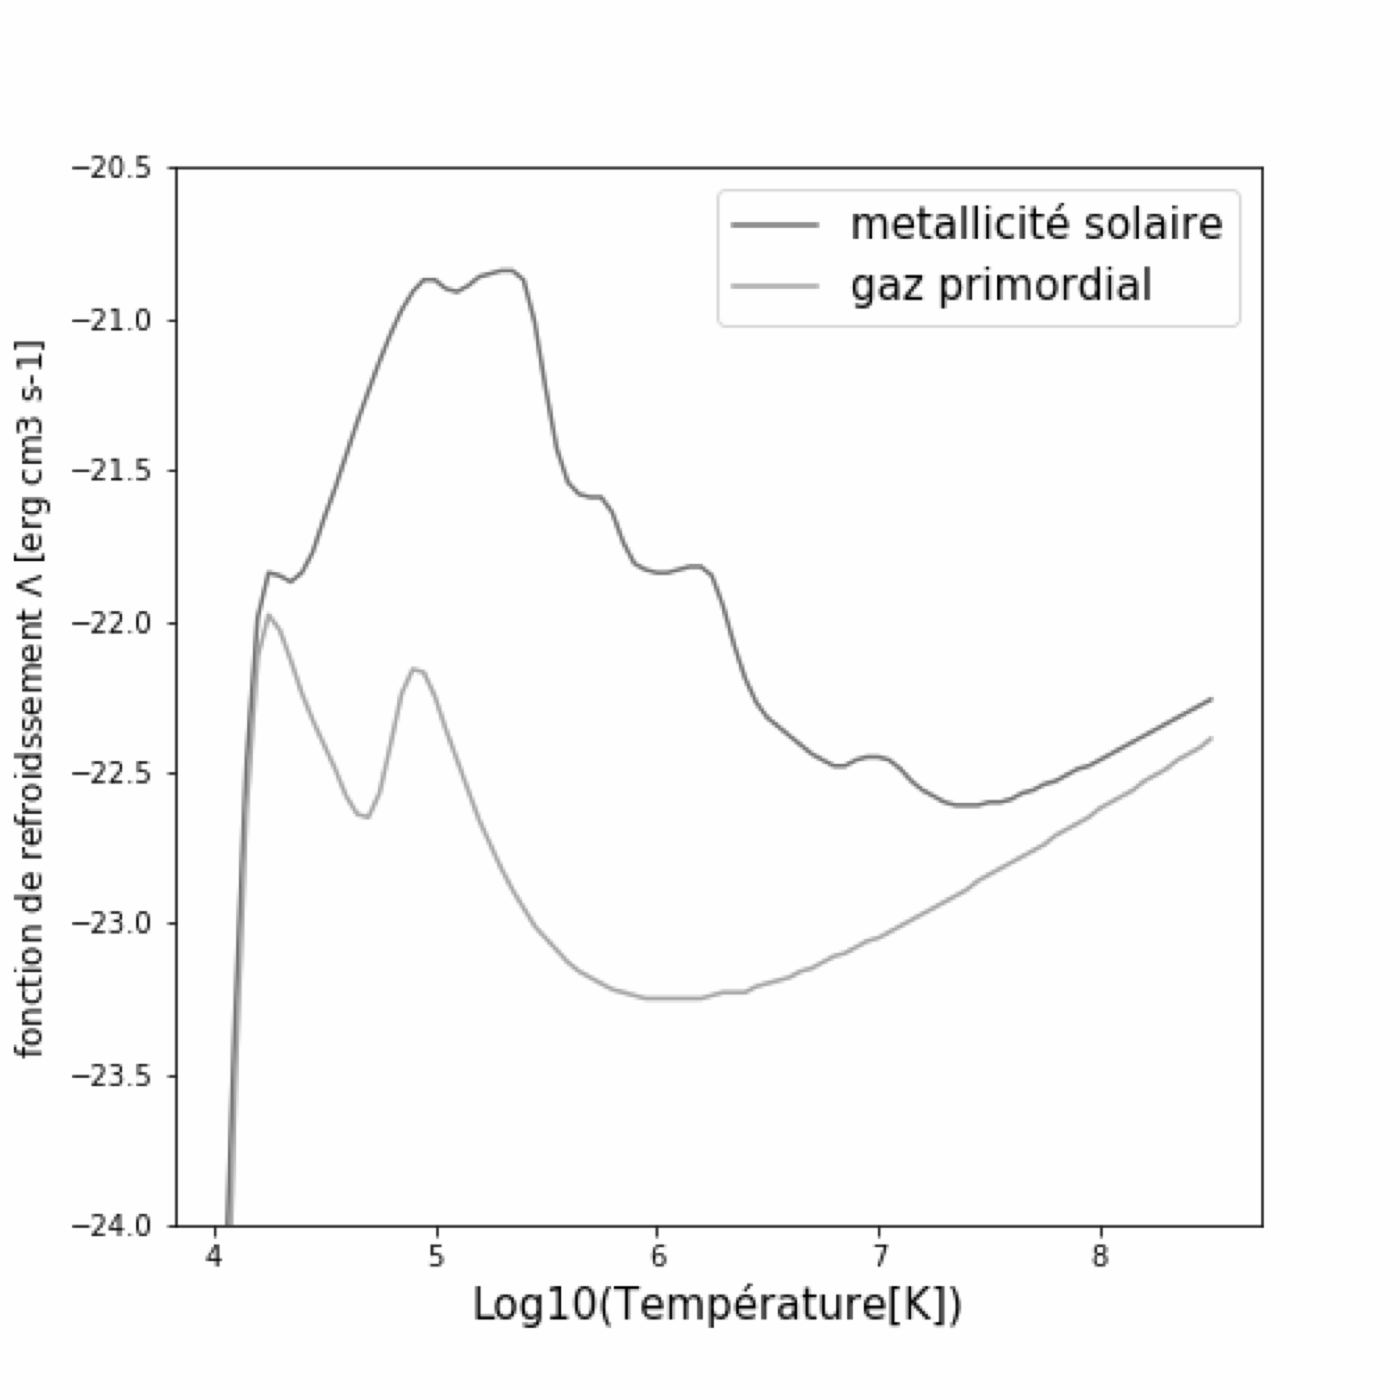
\includegraphics[height=10cm]{figs/cool.png}
		\caption[La fonction de refroidissement du gaz]{La fonction de refroidissement du gaz de Sutherland et Dopita, pour un gaz sans métaux, dit 'primordial' et un gaz avec une métallicité solaire. Dans les 2 cas, le refroidissement n'est efficace qu'au dessus de 10 000 K tandis que les hautes températures présente un comportement en $\sqrt{T}$ typique du Brehmstrahlung. Pour le gaz primordial on observe les 2 'bosses' caractéristiques des processus d'excitation collisionnelle de l'hydrogène et de l'hélium. Le gaz enrichi en métaux est globalement plus efficace car disposant des multiples canaux de refroidissement des éléments plus lourds que l'hélium. Les cas présentés ici supposent un équilibre d'ionisation.}
	\label{f:coolins}
\end{figure}


Pour finir, on a rapidement réalisé que lorsqu'il était actif, ce processus de refroidissement devenait trop efficace en particulier à grand redshift lorsque la matière était très dense, donnant des petites galaxies trop abondantes, un nombre trop important d'étoiles ou des galaxies de trop petites tailles, trop concentrées \sidenote{par exemple dans les travaux de White \& Rees à la fin des années 70 ou Navarro \& White dans les années 90s}. Il faut donc réinjecter de l'énergie dans le gaz pour qu'il arrête ce refroidissement catastrophique, via par exemple l'énergie injectée par les explosions d'étoiles en fin de vie en supernovæ\index{supernovæ} ou par la présence d'un fond de rayonnement ultra-violet\index{fond UV}. On reviendra sur ces sujets dans la partie dédiée aux simulations numériques.
